\documentclass{article}
\usepackage{tikz}
\usetikzlibrary{matrix}

\begin{document}

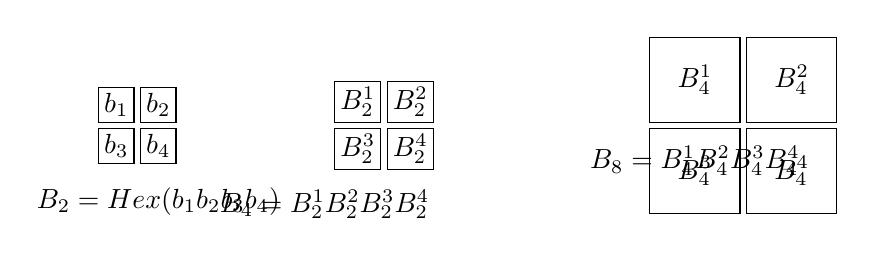
\begin{tikzpicture}

% Matrix for B2
\matrix[matrix of math nodes, anchor=west, row sep=2pt, column sep=2pt] at (0,0) {
  \node (b1) [draw, rectangle, inner sep=2pt] {b_1}; & \node (b2) [draw, rectangle, inner sep=2pt] {b_2}; \\
  \node (b3) [draw, rectangle, inner sep=2pt] {b_3}; & \node (b4) [draw, rectangle, inner sep=2pt] {b_4}; \\
};
\node[below=5pt] at (b4.south) {$B_2 = \text{Hex}(b_1 b_2 b_3 b_4)$};

% Matrix for B4
\matrix[matrix of math nodes, anchor=west, row sep=2pt, column sep=2pt] at (3,0) {
  \node [draw, rectangle, inner sep=2pt] {B_2^1}; & \node [draw, rectangle, inner sep=2pt] {B_2^2}; \\
  \node [draw, rectangle, inner sep=2pt] {B_2^3}; & \node [draw, rectangle, inner sep=2pt] {B_2^4}; \\
};
\node at (3,-1) {$B_4 = B_2^1 B_2^2 B_2^3 B_2^4$};

% Matrix for B8
\matrix[matrix of math nodes, anchor=west, row sep=2pt, column sep=2pt] at (7,0) {
  \node (topleft) [draw, rectangle, inner sep=10pt] {B_4^1}; & \node [draw, rectangle, inner sep=10pt] {B_4^2}; \\
  \node [draw, rectangle, inner sep=10pt] {B_4^3}; & \node [draw, rectangle, inner sep=10pt] {B_4^4}; \\
};
\node[below=5pt] at (topleft.south) {$B_8 = B_4^1 B_4^2 B_4^3 B_4^4$};

\end{tikzpicture}

\end{document}